\documentclass[10pt,a4paper,UTF8]{article}
\usepackage{zclorg}
\author{emacsun (所有文章遵循GPL协议)}
\date{\textit{[2015-05-08 Fri]}}
\title{LTE笔记概述}
\hypersetup{
 pdfauthor={emacsun (所有文章遵循GPL协议)},
 pdftitle={LTE笔记概述},
 pdfkeywords={},
 pdfsubject={},
 pdfcreator={Emacs 25.0.50.1 (Org mode 8.3.2)}, 
 pdflang={English}}
\begin{document}

\maketitle\xiaosihao
\tableofcontents\newpage\newpage

这是一系列LTE学习笔记,包括LTE物理层信号处理流程和UE接入流程等方面的知识。由于我本身就是学通信出身,对物理层的知识掌握更多一些,所以这些博文也更多的保函一些物理层的知识。我也在努力的扩展自己的知识面,尤其工作之后发现,仅仅掌握物理层的知识是远远不够的,就像构建自己的网站一样,仅仅懂一些javascript和css前端是不够的还需要了解一些后端数据库方面的东西。工作中出了吃物理层的老本之外,我还有意扩展通信资源管理,协议设计,随机接入等方面的知识。可以说一入通信深似海,从此偷懒是路人。这些博文也是我巩固已有知识,扩展未知领域的印记。

读了《大话移动通信》,让我明白,原来通信可以这么玩儿。作者深入浅出的表述让我折服,我也想让我的博文深入浅出。与《大话移动通信》不同,这些博文侧重于阐述通信知识中的"道"----在《大话移动通信》中,作者说:通信知识可以分两种:一种谓之"术",一种谓之"道"。"术"层面的知识是广大运维工程师需要用到的,运维工程师根据各种通信协议(2G协议,3G协议,4G协议等等等等),叮叮当当敲着键盘,焊着单板,调试系统。在这些协议的背后蕴含着一种叫做“道”的东西,这些东西是人类智慧的结晶,它们是通信的本质,展示了数学之美。正是这些“道”和“术”让通信行业成为理论和工程完美结合的典范,在这个行业中,拉光纤的也可以说是搞通信的,写协议栈的也可以说是搞通信的,坐实验室里matlab仿真算法的也可以说是搞通信的,总之好像跟手机电脑有些关系的都可以说是搞通信的。如果你不承认,人家还有点儿不开心。《大话移动通信》侧重于“术”的讲解,我则准备重点阐述通信的“道”。不过由于自己“道”行尚浅,难免表述不准,贻笑大方。不过幸亏我脸皮厚,欢迎指点。


\section{LTE物理层}
\label{sec:orgheadline1}


可以说物理层已死,也可以说物理层还顽强的活着。说物理层已死是因为近年来逼近香农极限的技术已经出现,并且不断的出现,远的说有LDPC,Turbo等信道编码,近的说有rateless。MIMO技术也不再是什么新鲜的技术,虽然massive-mimo可能火了一把,但也是新瓶装旧酒,可以说物理层领域的新技术泛善可陈。说物理层还顽强的活着,是因为还有很多具体的问题有待解决,比如虽然Turbo码和LDPC码已经逼近了香农极限,但是这两个码可都不是省油的灯,Turbo码虽然编码简单但是译码复杂,LDPC则相反。如何设计简单易用的编译码算法看起来是个工程问题,但是其背后蕴含深奥的数学原理。截至目前,这两种信道编码的译码都采用一种叫做和积算法的译码架构,这还没有考虑并行实现。再比如,MIMO技术的引入虽然增加了空域的自由度,但是多天线带来的复杂度也是指数级别的,如何降低解MIMO的计算复杂度一直以来都是研究的热点,尤其当massive-mimo技术提出以后,将复杂度的问题日益突出。另外,貌似所提的这些搞复杂度问题都某种程度上具有一定的可并行性,所以如何设计并行算法,充分利用当前过剩的硬件计算能力也是一个挑战。总之,物理层可做的事情还很多。

通信系统的物理层包含的模块都大同小异,区别在于为了满足不同的需求所采用的技术不同,比如信道编码模块有的采用分组码,有的采用卷积码;交织模块所采用的交织算法,不同通信系统也有所不同\ldots{}\ldots{}LTE的物理层其信号处理流程如图(\ref{fig:20150716LTEdownlink})所示:
\begin{figure}[htb]
\centering
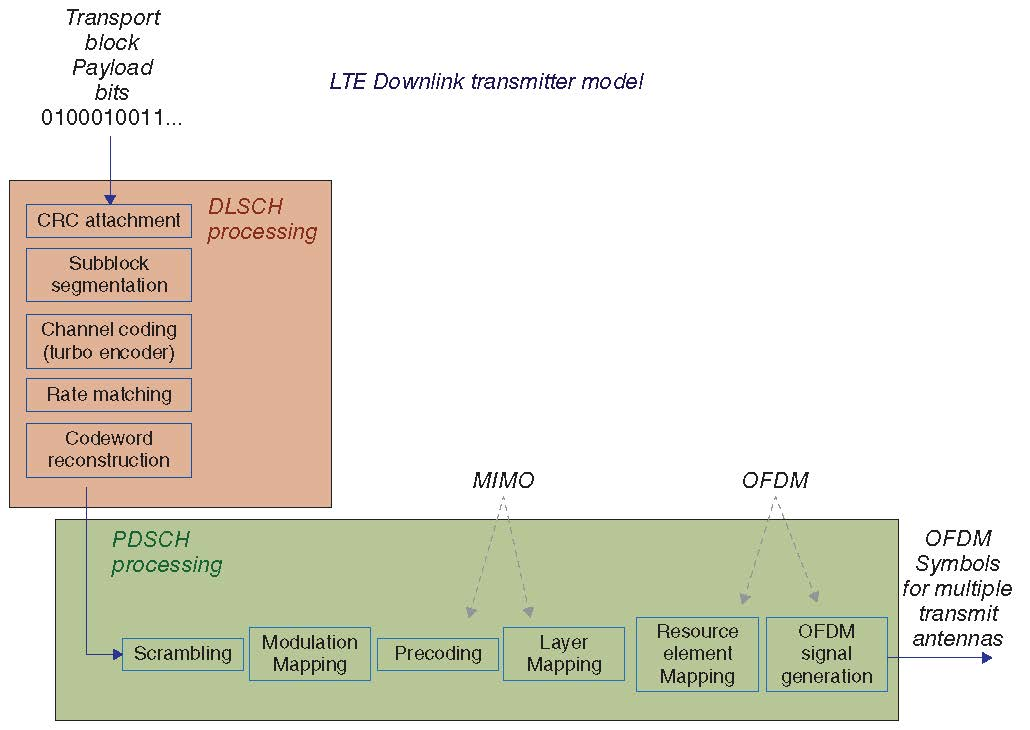
\includegraphics[width=0.5\textwidth]{../img/20150716LTEdownlink.jpg}
\caption{\label{fig:orgparagraph1}
LTE PDSCH物理层下行链路信号处理流程}
\end{figure}

\begin{itemize}
\item \href{physical/lte-physical-overview.org}{LTE 物理层技术概要}
\end{itemize}
\section{LTE接入}
\label{sec:orgheadline2}
\end{document}
